%!TEX root=paper.tex

\newpage
\section{Do The Readers Find Personally Interesting Articles?}

\subsection {Feed Subscriptions}
Figure \ref{fig:registrations} represents an incidence matrix collected at the end of the study interval: the columns represent students, and the rows represent news feeds; if a student is registered to a given feed, at the intersection of the corresponding row and column we place $\Diamond$. 

We would expect to see fully continuous horizontal rows of data-points if every user subscribed to the same feed, and fully continuous vertical rows if every user subscribed to all of the feeds available. The notion that these patterns are largely absent in Figure 4 supports our assumption that different individuals prefer to subscribe to different reading sources.

The figure illustrates that giving the students the freedom to choose the sources they wanted, allowed each one of them to express their interest. 

\begin{figure}[h!]
\centering
  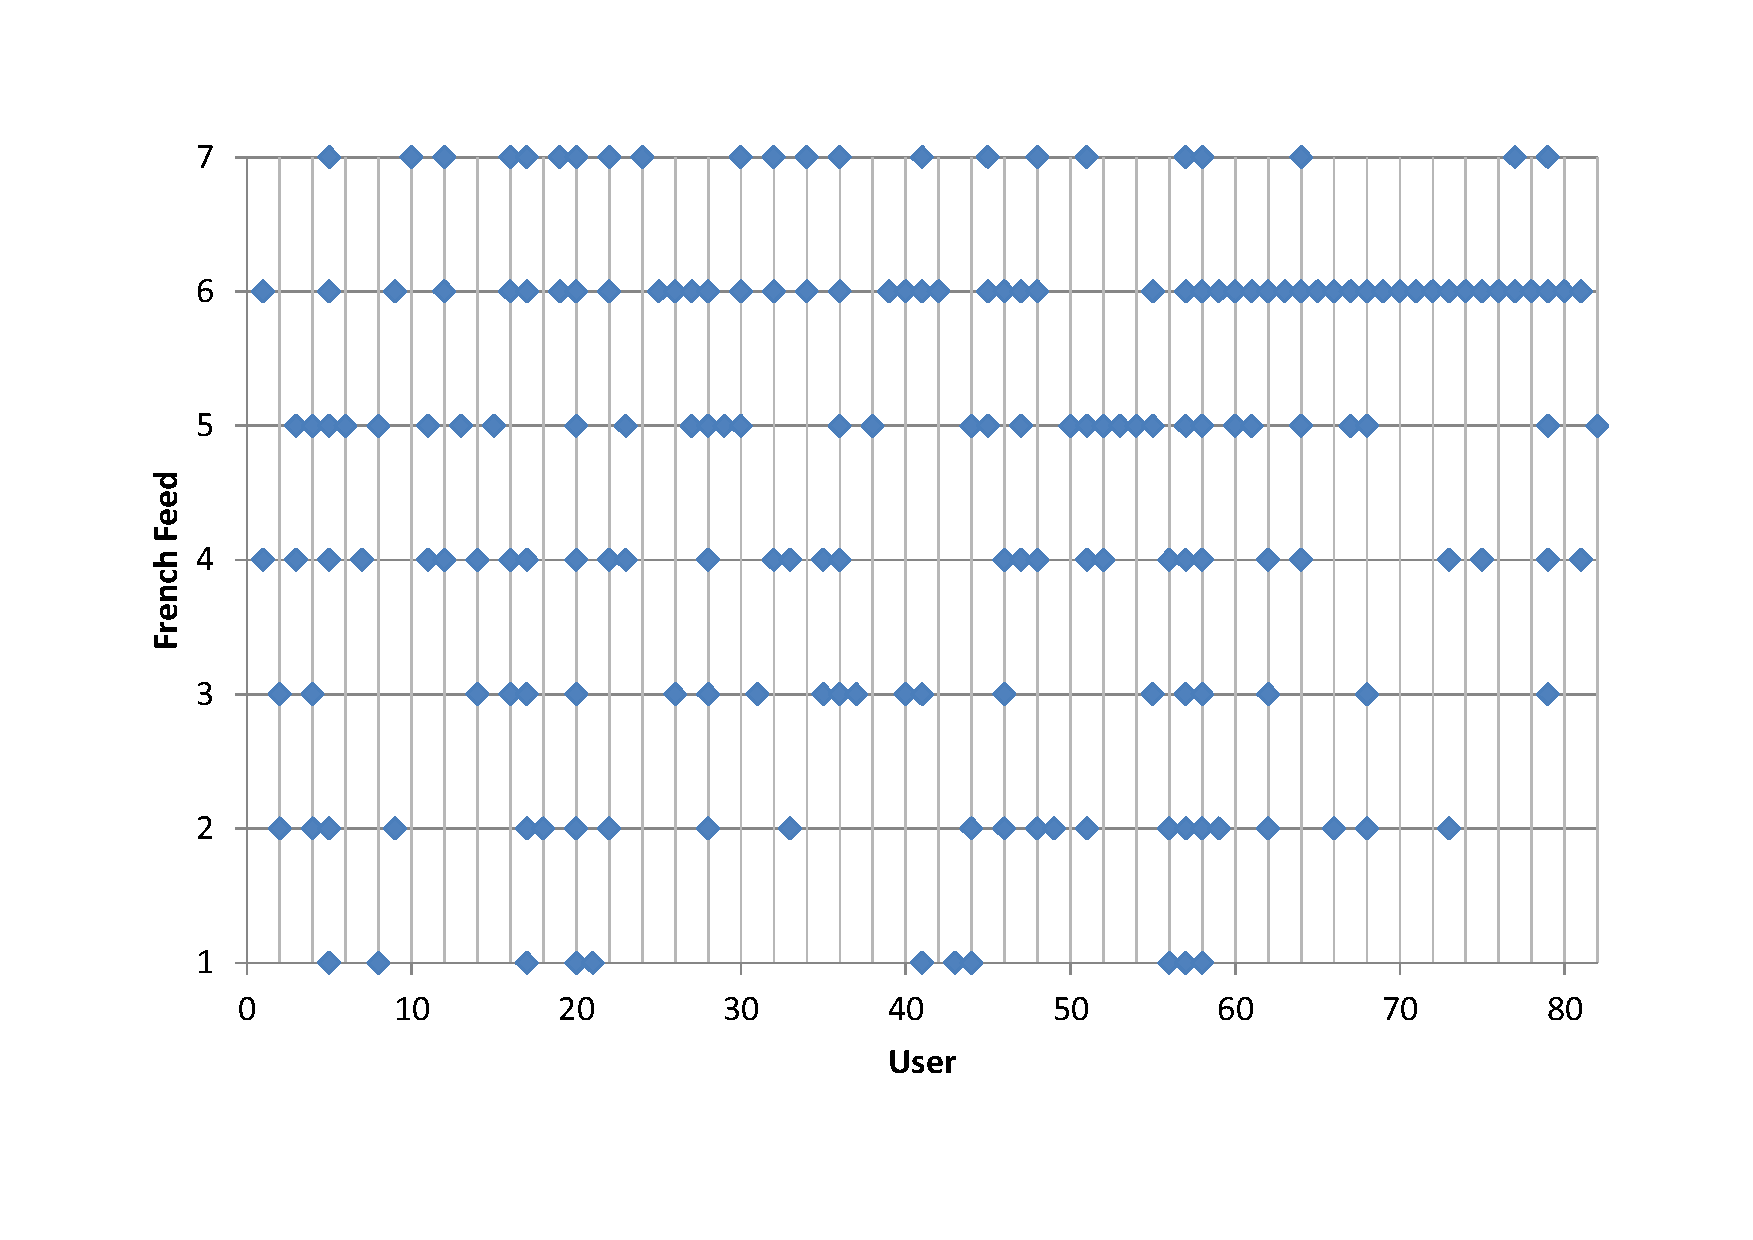
\includegraphics[width=\columnwidth]{figures/users_feeds}
  \caption{Different users subscribe to different sources}~\label{fig:registrations}
\end{figure}

Of course some feeds are more popular than others. Projecting the data- points into the vertical axis and sorting the results leaves us with a histogram as can be seen in Figure 5.

\begin{figure}[h!]
\centering
  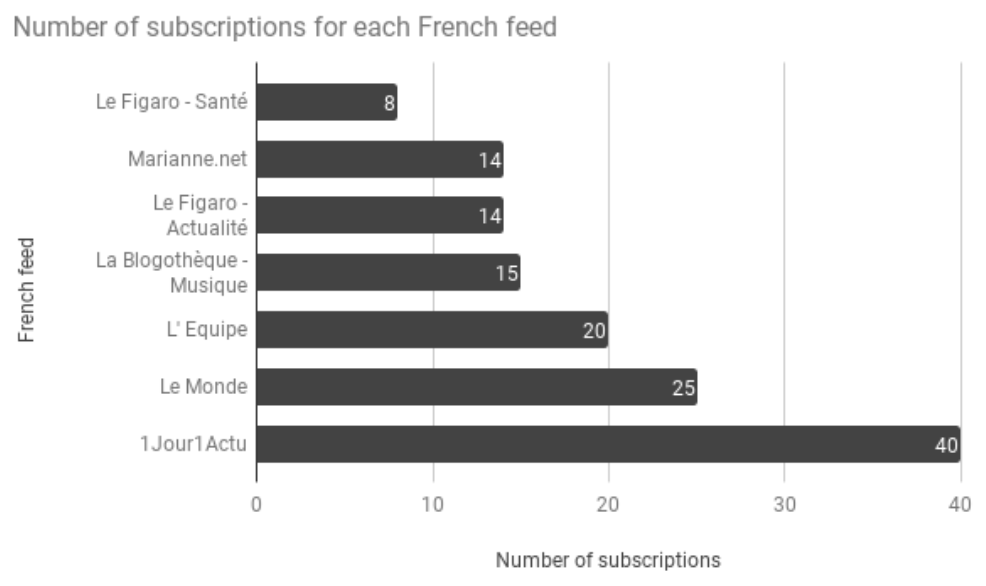
\includegraphics[width=\columnwidth]{figures/feed_popularity}
  \caption{Some feeds are more popular than others}~\label{fig:registrations}
\end{figure}


Feed {\em 1Jour1Actu} is the most popular French feed, and feed Le Figaro - Sant\'e is the least popular French feed. In order to see whether or not this might be related to how they are presented in the dialog window of our system (see Figure \ref{fig:system_subscriptions}), we can compare the order of popularity with the order in which they are displayed.

\begin{figure}[h!]
\centering
  \newcommand{\picscale}{0.5}
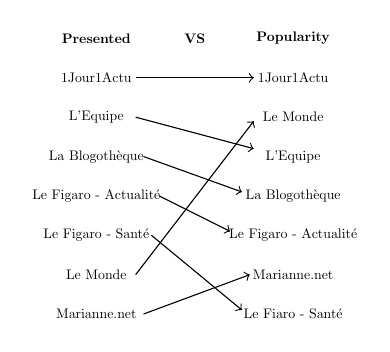
\begin{tikzpicture}[scale=\picscale, every node/.style={scale=\picscale}]
    % Columns.
    \node at (0  , 0) {\bf Presented};
    \node at (2.5, 0) {\bf VS};
    \node at (5  , 0) {\bf Popularity};
    
    % As presented.
    \node at (0,-1) {1Jour1Actu};
    \node at (0,-2) {L'Equipe};
    \node at (0,-3) {La Blogoth\`{e}que};
    \node at (0,-4) {Le Figaro - Actualit\'{e}};
    \node at (0,-5) {Le Figaro - Sant\'{e}};
    \node at (0,-6) {Le Monde};
    \node at (0,-7) {Marianne.net};
    
    % As popular.
    \node at (5,-1) {1Jour1Actu};
    \node at (5,-2) {Le Monde};
    \node at (5,-3) {L'Equipe};
    \node at (5,-4) {La Blogoth\`{e}que};
    \node at (5,-5) {Le Figaro - Actualit\'{e}};
    \node at (5,-6) {Marianne.net};
    \node at (5,-7) {Le Fiaro - Sant\'{e}};
    
    % Arrows between presented and popular.
    \draw [->] (1,-1)   --   (4,-1);
    \draw [->] (1,-2)   --   (4,-2.8);
    \draw [->] (1.2,-3) --   (3.7,-3.9);
    \draw [->] (1.6,-4) --   (3.4,-4.9);
    \draw [->] (1.4,-5) --   (3.7,-6.9);
    \draw [->] (1,-6)   --   (4,-2.1);
    \draw [->] (1.2,-7) --   (3.9,-6);
    
\end{tikzpicture} 
  \caption{The popularity of the feeds vs. their ranking in the UI}~\label{fig:registrations}
\end{figure}

One can see how the second-to-last presented feed, Le Monde, is the second most popular feed by measure of subscriptions. Conversely, the feed listed above Le Monde is actually the least subscribed-to feed in our listing.

\subsection{Article Interactions}
If we investigate the articles that the users interact with, we see the same pattern: each user explores their own interest, and there is no one article that is interesting for all of them. 

\begin{figure}[h!]
\centering
  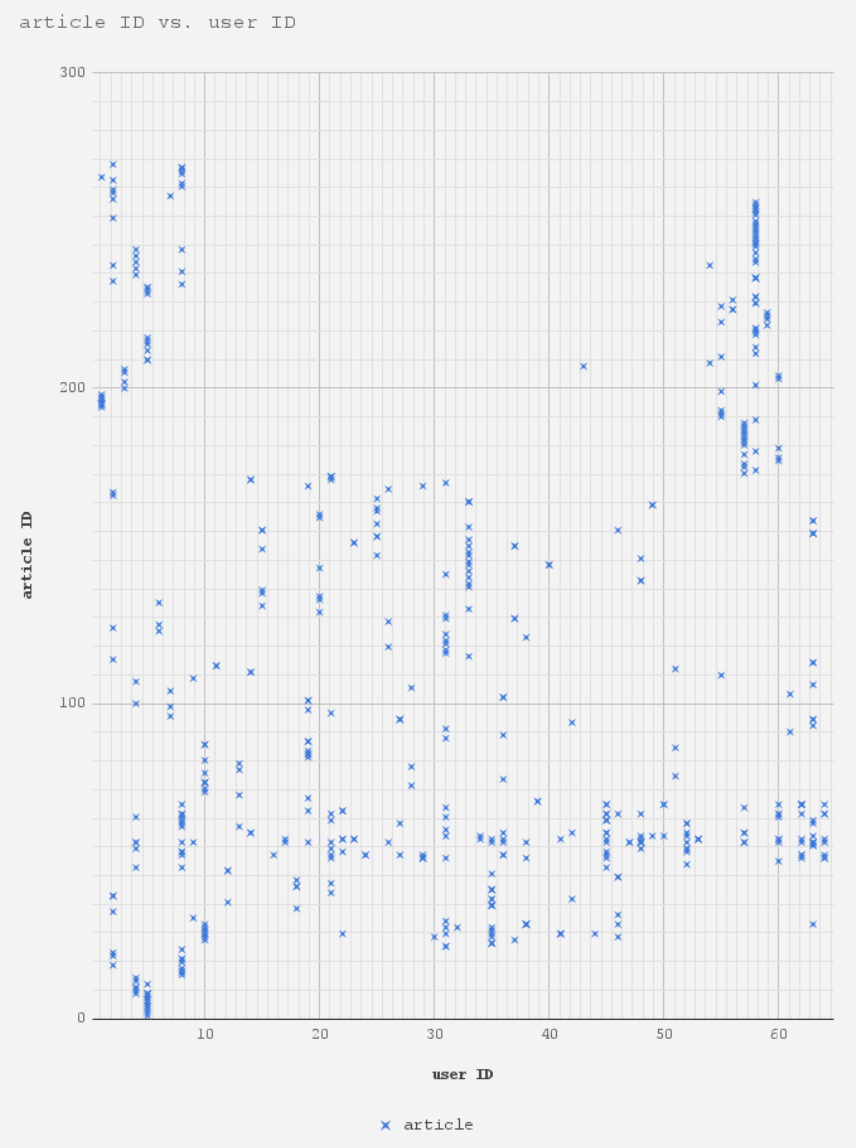
\includegraphics[width=\columnwidth]{figures/users_articles}
  \caption{Every student has their own article reading preferences}~\label{fig:registrations}
\end{figure}

\newpage
\section{Which of the Interactive Features Are Most Important When Reading?}
We tracked the usage of the various features in the interactive reader. What we see is that in average, a students requests an alternate translation for one in every eight translations. 

The third most used feature is the text to speech feature. This was a feature that was recommended by one of our expert beta-testers. 

\begin{figure}[h!]
\centering
  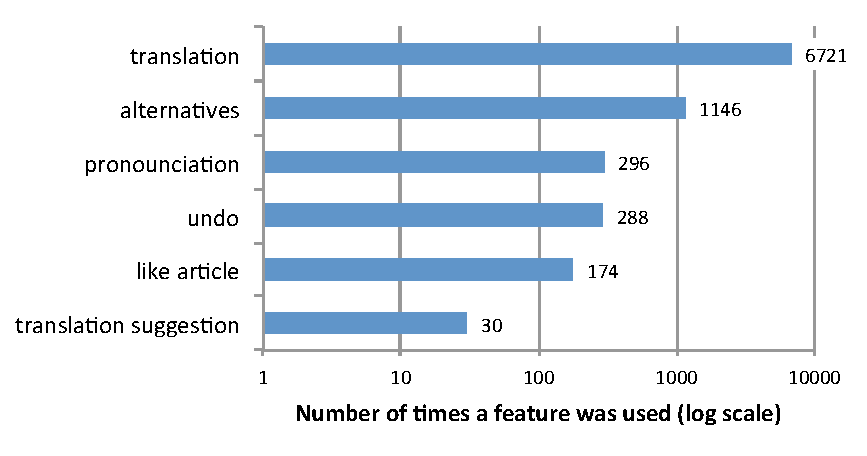
\includegraphics[width=0.9\columnwidth]{figures/reader_feature_usage}
  \caption{Popularity of features by their recorded usage-events}
\end{figure}
\todo{We should sort this graph similarly to the graph below. - Luc}

To see how widespread the various features are among our users, we also looked at the number of distinct users for each category of events. A larger number of distinct users indicates that the feauture is useful to the broadest number of students.

\begin{figure}[h!]
\centering
  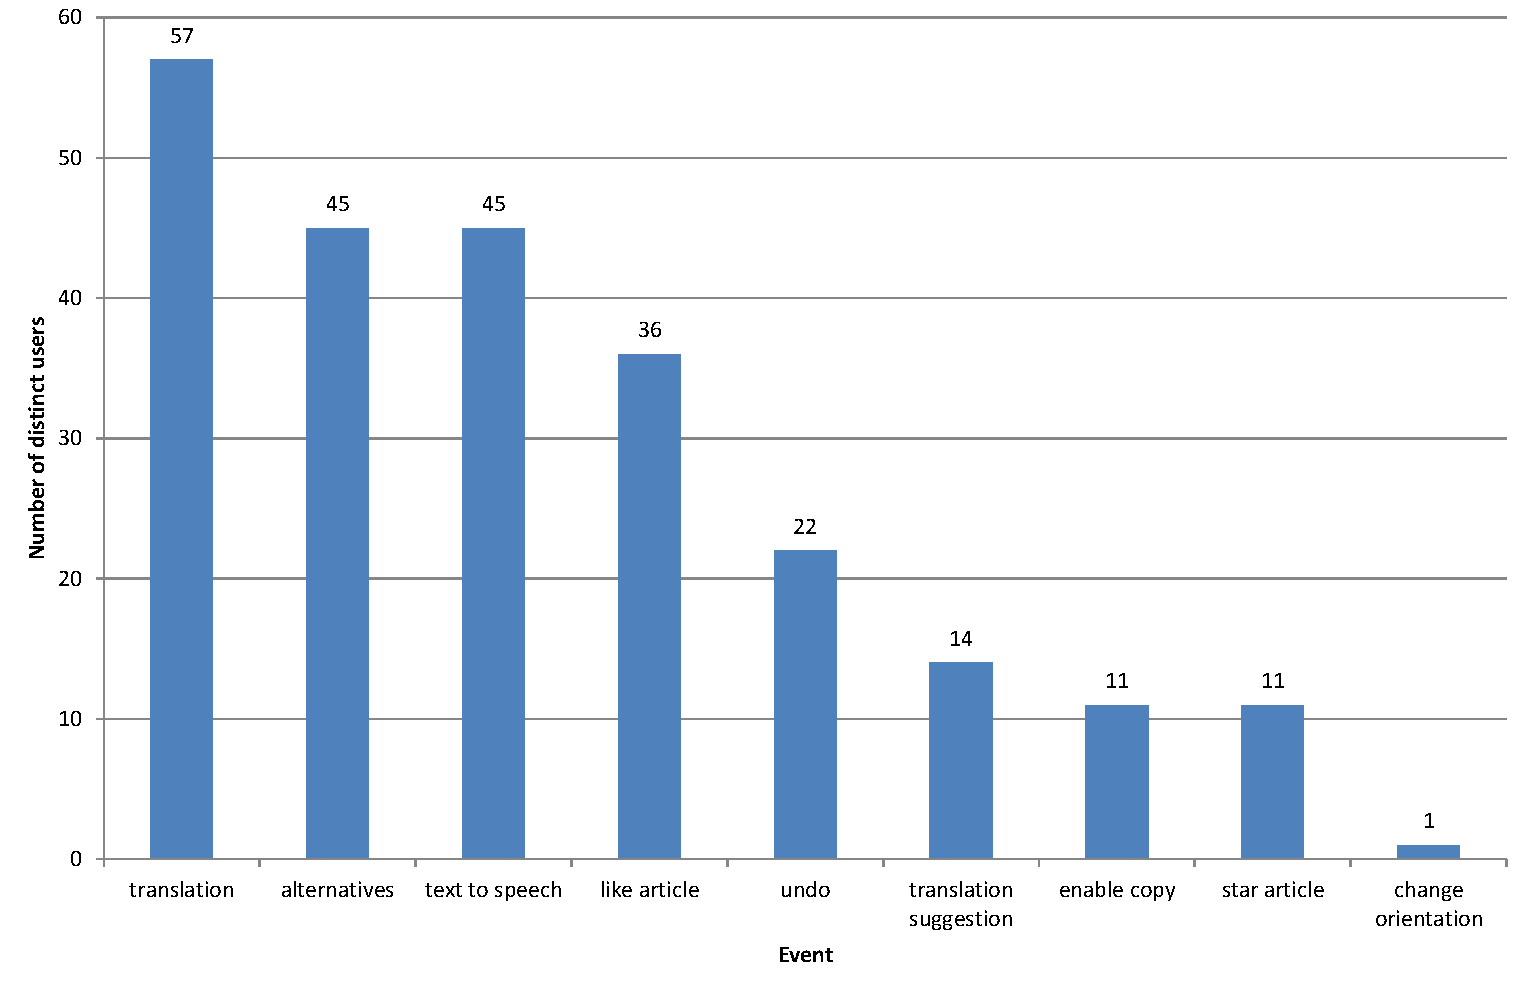
\includegraphics[width=0.9\columnwidth]{figures/reader_feature_usage_per_user}
  \caption{The usage of the various reader features by the various users }
\end{figure}

In addition, we looked at the number of times the same word or phrase was pronounced by the same user. This data ranges from one single pronunciation to 14 pronunciations for the same word (phrase). The size of this interval is mostly due to the users' different proficiency in a certain language and the difficulty in pronunciation of the word (phrase) itself. Nevertheless, on average, the number approaches 1.66 pronunciation requests for the same
piece of text, suggesting that users are generally sufficiently content with a pronunciation after hearing it the first time.



\section{Are the Personalized Exercises Useful?}

The personalized exercises are a complement to the reading. To show that 
users actually use them ... 

\begin{figure}[h!]
\centering
  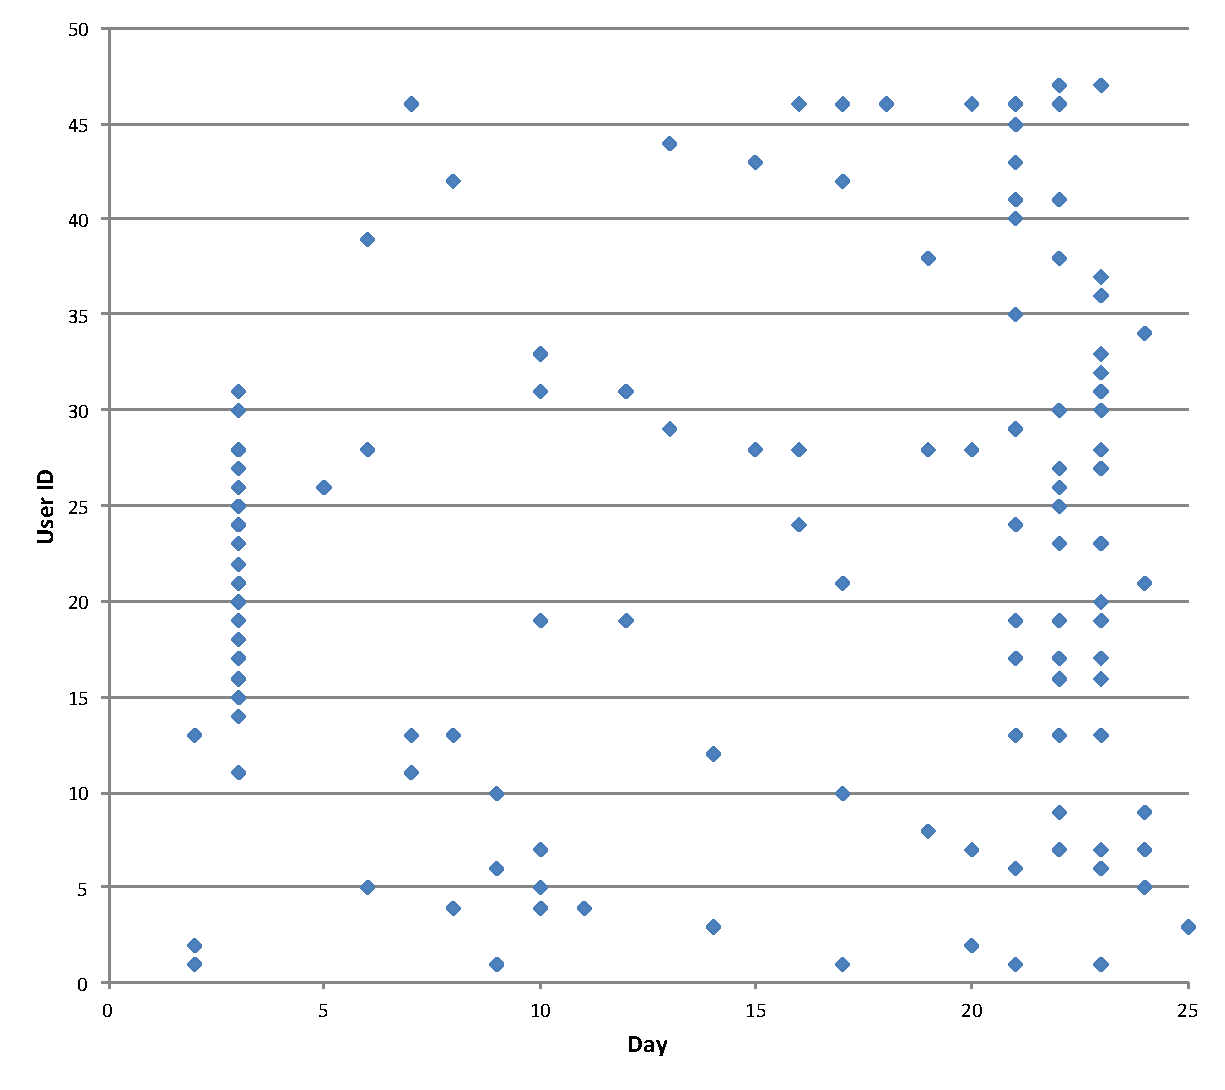
\includegraphics[width=\columnwidth]{figures/user_exercise_activity_vs_day.pdf}
  \caption{The students are doing exercises at their own pace throughout the one month interval }
\end{figure}

we could also show that they benefit from them... 



\section{User Feedback}

Besides the analysis that we did based on the observed user data, we also asked the students a series of questions, among which whether they preferred the reading platform and why. Some of the qnswers can be seen in the screenshot below. It becomes clear that the students appreciate the possibility of reading what is interesting for them.


\section{Threats to Validity}

Threat to external validity: we believe that the students we worked with are representative for the Dutch highschool student population. 

We presented a system, and we showed that it has the potential to generate user involvement. However the study we performed is not sufficient to reach a strong conclusion about the impact of the system we present... 

The feedback from the users was positive. However, they might have been influenced by our enthusiastic presentation of the system at the begining of the testing month. 

We showed that the users are using the system extensively. However, this might be because the students had to use the system as part of their assignment in the class. We showed that the majority of the students used the system constantly throughout the one month period. If they only used it for a grade, we would have expected a more focused cramming at the end of the period (which we actually saw with a few of the students, but not with the majority). 

The majority of the students who answered our post-usage survey said that  they prefer our system to a textbook. However, we still think this is not very conclusive since the number of students who answered our survey was quite limited: 12 of the 60 students represent about 20\% of the participants. 

% We observed that students prefer to interact with different texts...  

The algorithms for scheduling are the state of the art in spaced repetition. However, we did not have a control group to see whether this approach works better than others. Moreover, note that other approaches for using spaced repetition already exist; what is unique in our approach is that the students learn based on personalized exercises generated based on the context of their past readings.


\section{Availability}
The system described in this paper is deployed online and available at \url{https://zeeguu.unibe.ch}. If the reader of this article would want to test it they are invited to use the ``CHI'' code word while following the  ``Become a Betatester'' link from the homepage.

\begin{figure}[h!]
\centering
  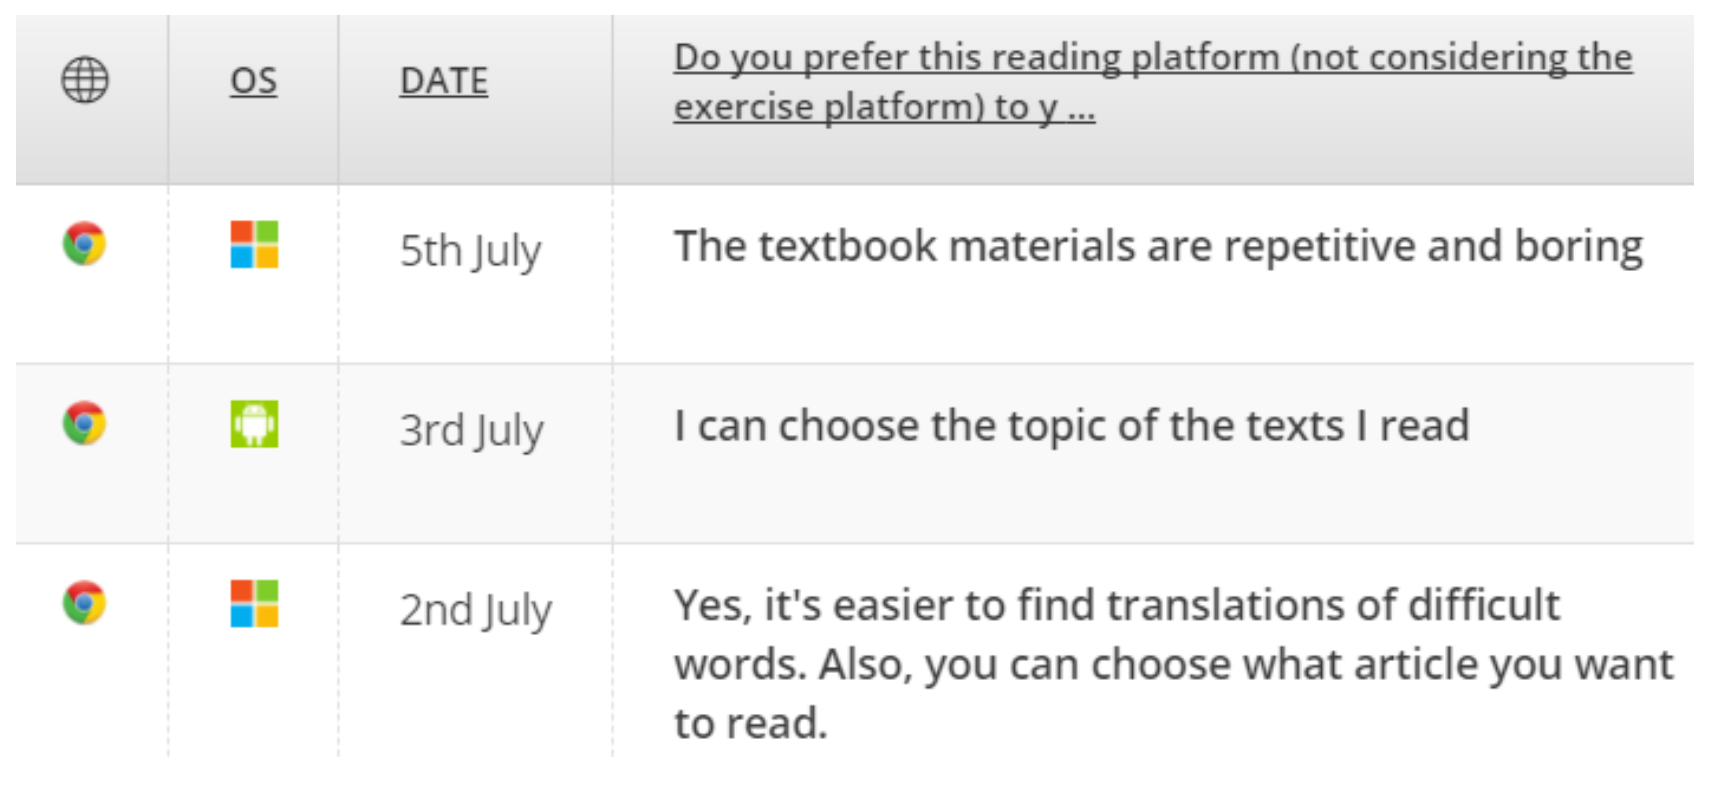
\includegraphics[width=0.9\columnwidth]{figures/opinion_on_reading_platform}
  \caption{The students appreciate the freedom of reading what is interesting to them }
\end{figure}

% \section{Acknowledgements}
% The authors would like to thank other contribu








